\section{Results}\label{sec:results}
\subsection{Voltage controlled voltage source (VCVS)}\label{sec:vcvs}
\begin{figure}[tbph]
	\centering
	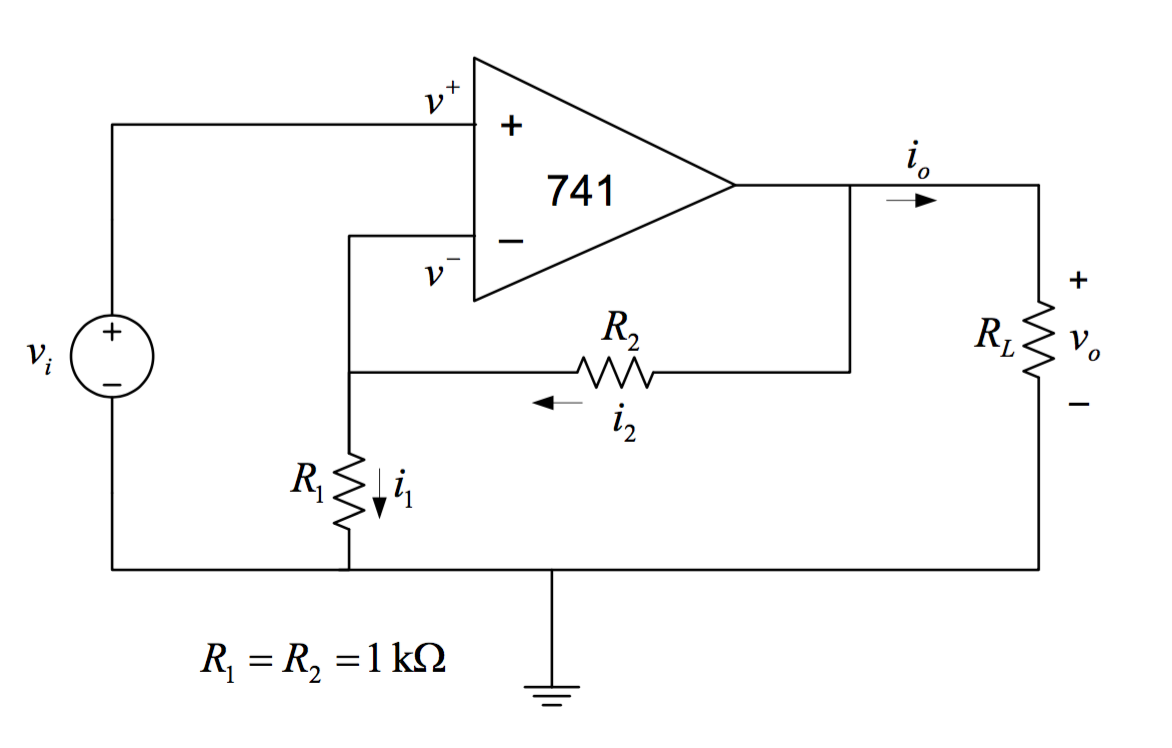
\includegraphics[width=0.7\linewidth]{graphics/vcvs-schematic}
	\caption{Schematic for VCVS with $K = 2$}
	\label{fig:vcvs-schematic}
\end{figure}

The voltage controlled voltage source acted as a linear function of the input voltage, with a slope of 2, between $-4.2\si{\volt}<V_i<4.5\si{\volt}$. The calculated linear region was between $-5\si{\volt}<V_i<5\si{\volt}$, which is close to our experimental results when accounting for the ignored output resistance. Our calculated value of 2 for K (the gain) agrees with the results we observed.

\begin{table}[htpb]
	\centering
	\begin{tabular}{@{}SS@{}}
		\toprule
		\textcol{$V_i$ (\si{\volt})} & \textcol{$V_o$ (\si{\volt})} \\ \midrule
		-6 & -8.467 \\
		-5 & -8.468 \\
		-4 & -8.007 \\
		-3 & -6.005 \\
		-2 & -4.003 \\
		-1 & -2.001 \\
		0 & 0.001 \\
		1 & 2.036 \\
		2 & 4.007 \\
		3 & 6.010 \\
		4 & 8.011 \\
		5 & 9.060 \\
		6 & 9.060 \\ \bottomrule
	\end{tabular}
	\caption{Response of VCVS}
	\label{table:vcvs}
\end{table}

\begin{figure}
	\centering
	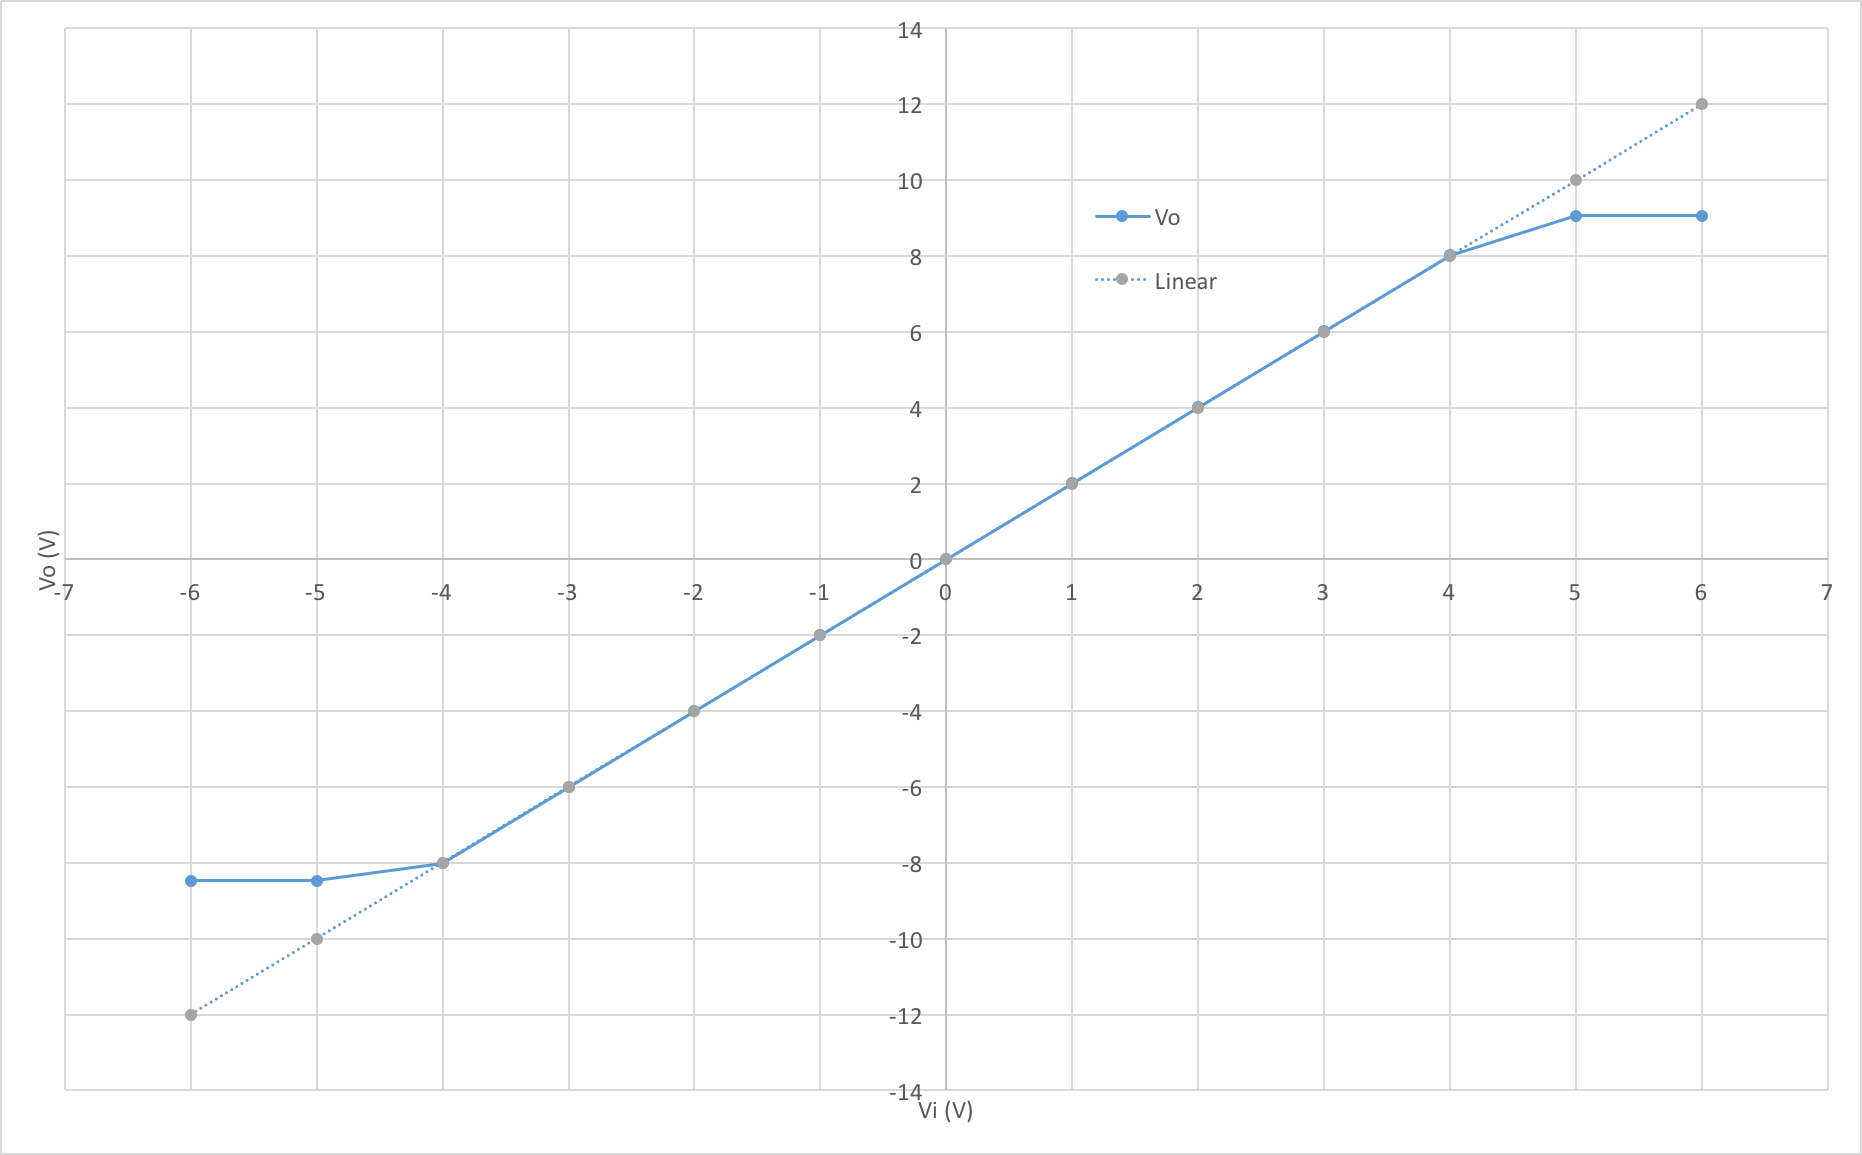
\includegraphics[width=0.7\linewidth]{graphics/vcvs-graph}
	\caption{Response characteristic of VCVS with expected linear behavior}
	\label{fig:vcvs-graph}
\end{figure}

When we attempted to estimate the internal resistance using a 150\si{\ohm} load ($R_L$ in Fig.~\ref{fig:vcvs-schematic}, we were only receiving a drop in voltage of approximately 6\si{\micro\volt} (peak-to-peak), which implied an internal resistance of approximately 500\si{\micro\ohm}: this was considered to be incorrect. Replacing the 150\si{\ohm} load with a 47\si{\ohm} load, we experienced a more plausible result. With a load of 47\si{\ohm}, the voltage across the load was measured to be 788.5\si{\milli\volt}, which means the source has an estimated internal resistance of approximately 39.1\si{\ohm} (see~\ref{eq:internal-resistance}).

\begin{equation}
	I_o	= \frac{V_o}{R_L} = \frac{0.7885\si{\volt}}{47\si{\ohm}} = 16\si{\milli\ampere}
\end{equation}
\begin{equation}
	V_{internal}		= V_i - V_L = 1.4135\si{\volt} - 0.7885\si{\volt} = 625\si{\milli\volt}
\end{equation}
\begin{equation}
	\label{eq:internal-resistance}
	R_{internal}	= \frac{V_{internal}}{I_o} = \frac{625\si{\milli\volt}}{16\si{\milli\ampere}} = 39.1\si{\ohm}
\end{equation}


\subsection{Voltage controlled current source (VCCS)}\label{sec:vccs}
\begin{figure}[tbph]
	\centering
	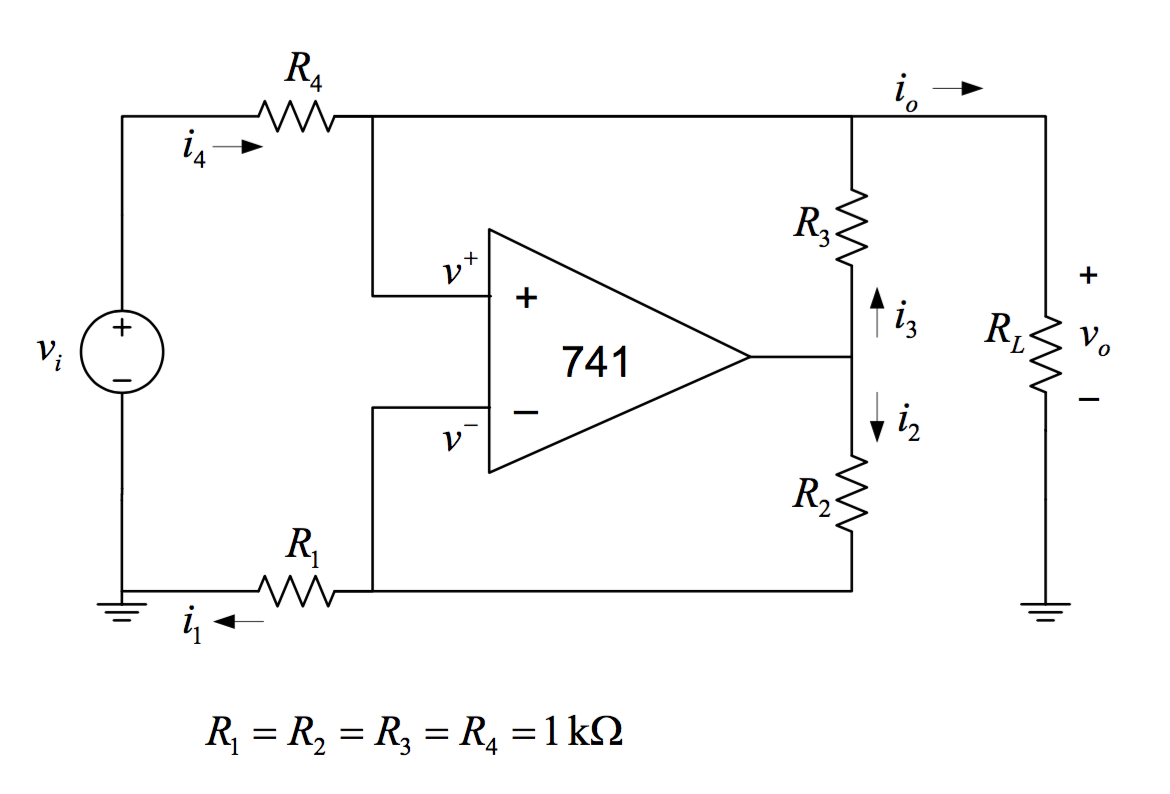
\includegraphics[width=0.7\linewidth]{graphics/vccs-schematic}
	\caption{Schematic for VCCS with $G = \frac{1}{1000}$}
	\label{fig:vccs-schematic}
\end{figure}

Evaluating the inequality (1.15)~\cite{lab-manual} gives $-5\si{\volt} V_i < 5\si{\volt}$, whereas we observed a linear region between approximately $-4.0\si{\volt}<V_i<4.2\si{\volt}$. When the edge of the linear region was reached, rather than hard limiting the current experience soft limiting where $G$ dropped to \num{328e-6}.

When shorting the output carrying 1\si{\milli\ampere} when measured under a 1\si{\kilo\ohm} load, the measured current dropped to 0.951\si{\milli\ampere}.

\large{\textit{Add a internal resistance calculation. Not sure how to do this eq'n.}}

Measuring the voltage between the inverting and non-inverting gives a reading of 0.97\si{\milli\volt}. In comparison to other voltages within the circuit and considering the immense input impedance, the current into each pin is indeed nearly non-existent and certainly negligible.

\begin{table}[htpb]
	\centering
	\begin{tabular}{@{}SS@{}}
		\toprule
		\textcol{$V_i$ (\si{\volt})} & \textcol{$I_o$ (\si{\milli\ampere})} \\ \midrule
		-8 & -5.405 \\
		-7 & -5.076 \\
		-6 & -4.747 \\
		-5 & -4.418 \\
		-4 & -4.056 \\
		-3 & -3.043 \\
		-2 & -2.028 \\
		-1 & -1.014 \\
		0 & -0.001 \\
		1 & 1.104 \\
		2 & 2.024 \\
		3 & 3.042 \\
		4 & 4.056 \\
		5 & 4.638 \\
		6 & 4.956 \\
		7 & 5.293 \\
		8 & 5.620 \\ \bottomrule
	\end{tabular}
	\caption{Response of VCCS}
	\label{table:vccs}
\end{table}

\begin{figure}[tbph]
	\centering
	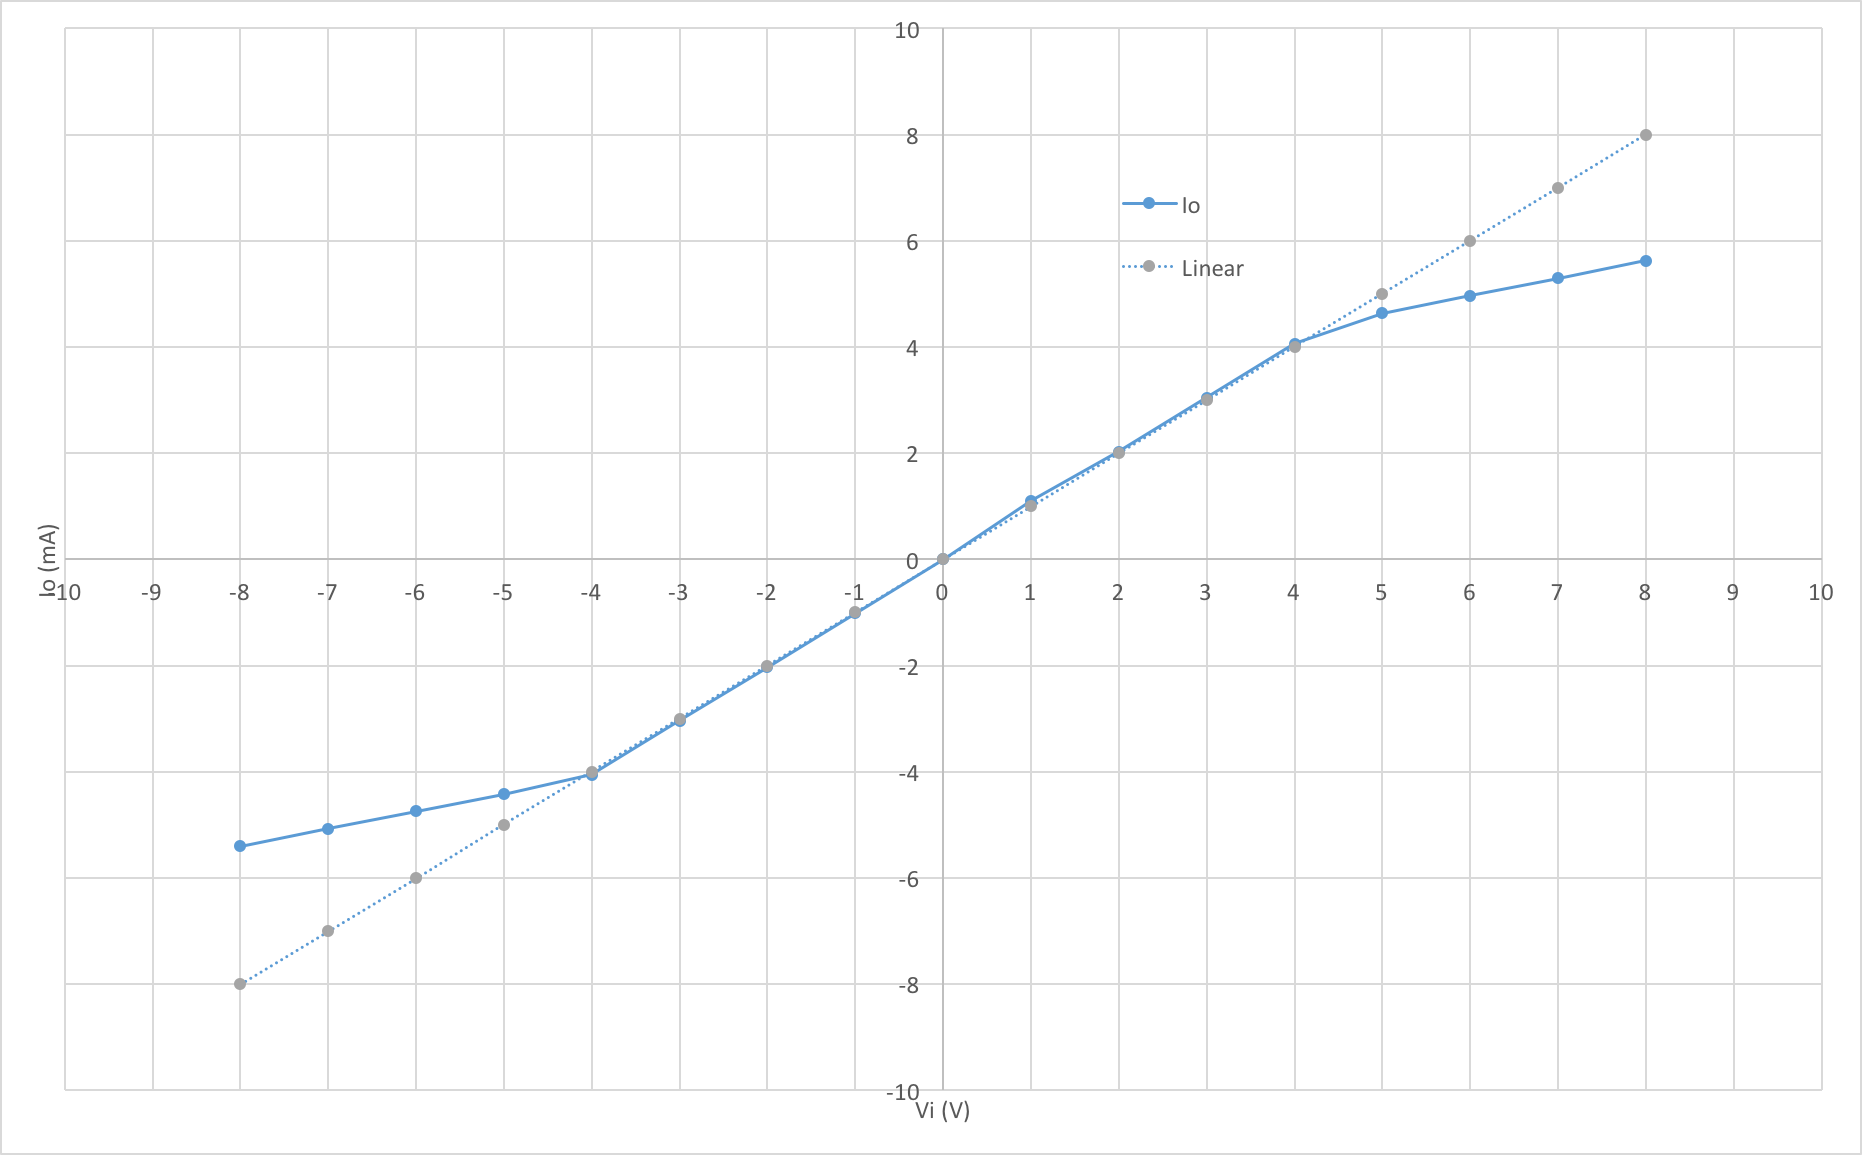
\includegraphics[width=0.95\linewidth]{graphics/vccs-graph}
	\caption{Response characteristic of VCCS with expected linear behavior}
	\label{fig:vccs-graph}
\end{figure}
